\chapter{Математический минимум}
\subsection*{Обозначения}
\begin{description}
\item[$\in$] --- принадлежит
\item[$\subset$] --- является подмножеством,
\item[$\forall$] --- для любого,
\item[$\exists$] --- существует,
\item[$\Rightarrow$] --- следует,
\item[$|\cdot|$] --- абсолютное значение (модуль),
\item[$\amalg$] --- пусть (квантор попустительства).
\end{description}
\section{Функции}
\begin{definition}[Функция]
Пусть есть числовые множества $X=\mathbb{D}(f) \subset \mathbb{R}$ 
(область определения) и $Y=\mathbb{E}(f) \subset \mathbb{R}$ (множество
значений). Каждому $x\in X$ сопоставим \textbf{единственный} $y\in Y$.
\end{definition}
\begin{definition}[Полный образ функции]
$$\mathbf{Im} f = \{ f (x)~|~\forall x \in X \}$$
\end{definition}
\begin{definition}[Наложение (сюръекция)]
$$Y=\mathbf{Im} f$$
\end{definition}
В дальнейшем под словом <<функция>> будем подразумевать наложение. Если область определения
функции явно не указана, то будем подразумевать под $X$ естественную область определений ---
множество таких $x \in \mathbb {R}$, что выражение $f(x)$ определено.
\begin{definition}[Чётная функция]
$$\forall x \in X \Rightarrow -x \in X $$
$$f(x) = f(-x)$$
\end{definition}
\begin{example}[Пример чётных функций]
$$x^{2k},~k\in \mathbb{Z};~\cos x;~\ch x $$
\end{example}
\begin{definition}[Нечётная функция]
$$\forall x \in X \Rightarrow -x \in X $$
$$f(-x) = -f(x)$$
\end{definition}
\begin{example}[Пример нечётных функций]
$$x^{2k-1},~k\in\mathbb{Z};~\sin x;~\sh x $$
\end{example}
\begin{definition}[Монотонно возрастающая функция]
$$x_1~,x_2 \in X,~x_1 < x_2 \Rightarrow f(x_1) < f(x_2)$$
\end{definition}
Аналогичным образом определяются монотонно  убывающая функция, невозрастающая и неубывающая функции.
\begin{definition}[Абсолютный максимум]
$$x_0 \in X,~\forall x \ne x_0 f(x) < f(x_0)$$
\end{definition}
\begin{definition}[Локальный максимум]
$$x_0 \in X,~x\in \mathbb{B} (x_0,\varepsilon),~\varepsilon > 0,~ f(x) < f(x_0),$$
где $\mathbb{B}(x_0,\varepsilon) = \{x \in X~|~x \ne x_0,~|x-x_0|<\varepsilon\}$
\end{definition}
Аналогично определяются абсолютный и локальный минимумы.
\begin{definition}[Обратная функция]
Если каждому значению $y \in Y$ функции $f$ соответствует не более одного (в случае наложения --- строго
один) $x \in X$, то можно постороить обратную функцию по следующему правилу:
$$\mathbb{D}f^{-1} = \mathbf{Im}(f)$$
$$\mathbb{E}f^{-1} = \mathbb{D}f$$
$$\forall y \in \mathbb{E}f,~f^{-1}(y)=x,~x \in X,$$
при этом
$$y=f(x)$$
\end{definition}
\begin{definition}[Периодическая функция]
Если $$\exists \xi > 0~|~\forall x \in X,~f(x+\xi)=f(x),$$
то функцию $f$ называют периодической, а $\xi$ --- периодом.
\end{definition}
\subsection*{Задачи}
\begin{task}
Найдите естественную область определений следуюущих функций:
$\frac{1}{a^2-x^2};$
$\frac{1}{a^2-(x-b)^2};$
$\frac{1}{a^2+(x-b)^2};$
$\frac{1}{a-\sqrt{x-b}},$ $a,~b \in \mathbb{R}.$
\end{task}
\begin{solution}
$x\in \mathbb{R},~x \ne \pm a; $
$x \in \mathbb{R},~x \ne \pm a+b; $
$x \in \mathbb{R};$
$x \in \mathbb{R},~x \ge b,$ в случае
$a \ge 0 \Rightarrow x \ne a^2 + b.$
\end{solution}
\begin{task}
Найдите полный образ следующих функций:
$f(x)=\frac{1}{a^2 + (x-b)^2},$
$f(x)=\frac{1}{a + \sqrt{x-b}},$
$f(x)=\frac{\sqrt{x-a}}{\sqrt{x-b}}.$
\end{task}
\begin{solution}
Задача с нахождением области значений 
\textit{непрерывной} функции
обычно сводится к нахождению
абсолютного минимума и максимума функции.
\begin{enumerate}
\item $f(x)$ можно представить как композицию функций $\frac {1}{x}$ и
$a^2 + (x-b)^2.$
Минимальное значение выражение
${a^2 + (x-b)^2}$ принимает при $x=b,$ максимальное значение
не существует, функция неограничена сверху. Значит $f(x)$ ограничена
снизу нулём.
Поэтому окончательно получаем
$Y=\{x\in\mathbb{R}~|~0<x\le \frac{1}{a^2}\}.$
\item Аналогично предыдущему пункту задачи рассмотрим сначала множество значений
знаменателя. Ясно, что это полуось $[a,~+\infty).$ В зависимости от того, содержит
ли ноль это множество, возникает два случая. Если $a>0$, то знаменатель в ноль
не обращается, функция непрерывна, её множество значений $(0,~\frac{1}{a}].$
Если $a=0$, то имеем $Y=(0,~+\infty).$
В случае $a<0$ разобьём множество значений на две части: знаменатель больше нуля
(это соответствует множеству $(0,~+\infty)$) и знаменатель меньше нуля
(соответствует $(-\infty,~\frac{1}{a}],$ где окончательно получим
$Y=(-\infty,~\frac{1}{a}]\cup(0,~+\infty).$
\item Случай $a=b$ тривиален, $Y=\{1\}.$ Случай $a>b$ рассмотрим подробнее.
Рассмотрим подкоренное выражение
($x\in X$). $$\frac{x-a}{x-b} = 1 - \frac {a-b}{x-b}<1.$$
Подкоренное выражение монотонно возрастает, значит монотонно возрастает и корень
из него (на области определений). Поэтому имеем $Y=[0,1).$ Если $a<b,$ то
подкоренная функция (а следовательно и сама функция) монотонно убывает на $X.$
В этом случае имеем $Y=(1,+\infty).$
\end{enumerate}
\end{solution}
\begin{task}
Найдите функцию, обратную $f(x)=ax^2+bx+c.$
\end{task}
\begin{solution}
Если за $X$ выбрать $[-\frac{b}{2a},~+\infty),$
то $f^{-1}(x) = \frac{-b+\sqrt{b^2-4a(c-x)}}{2a}$.
Если за $X$ выбрать $(-\infty,~-\frac{b}{2a}],$
то $f^{-1}(x) = \frac{-b-\sqrt{b^2-4a(c-x)}}{2a}$.
\end{solution}
\section{Тригонометрические функции}
Рассмотрим окружность единичного радиуса.
\begin{wrapfigure}{r}{0.5\textwidth}
 \begin{center}
  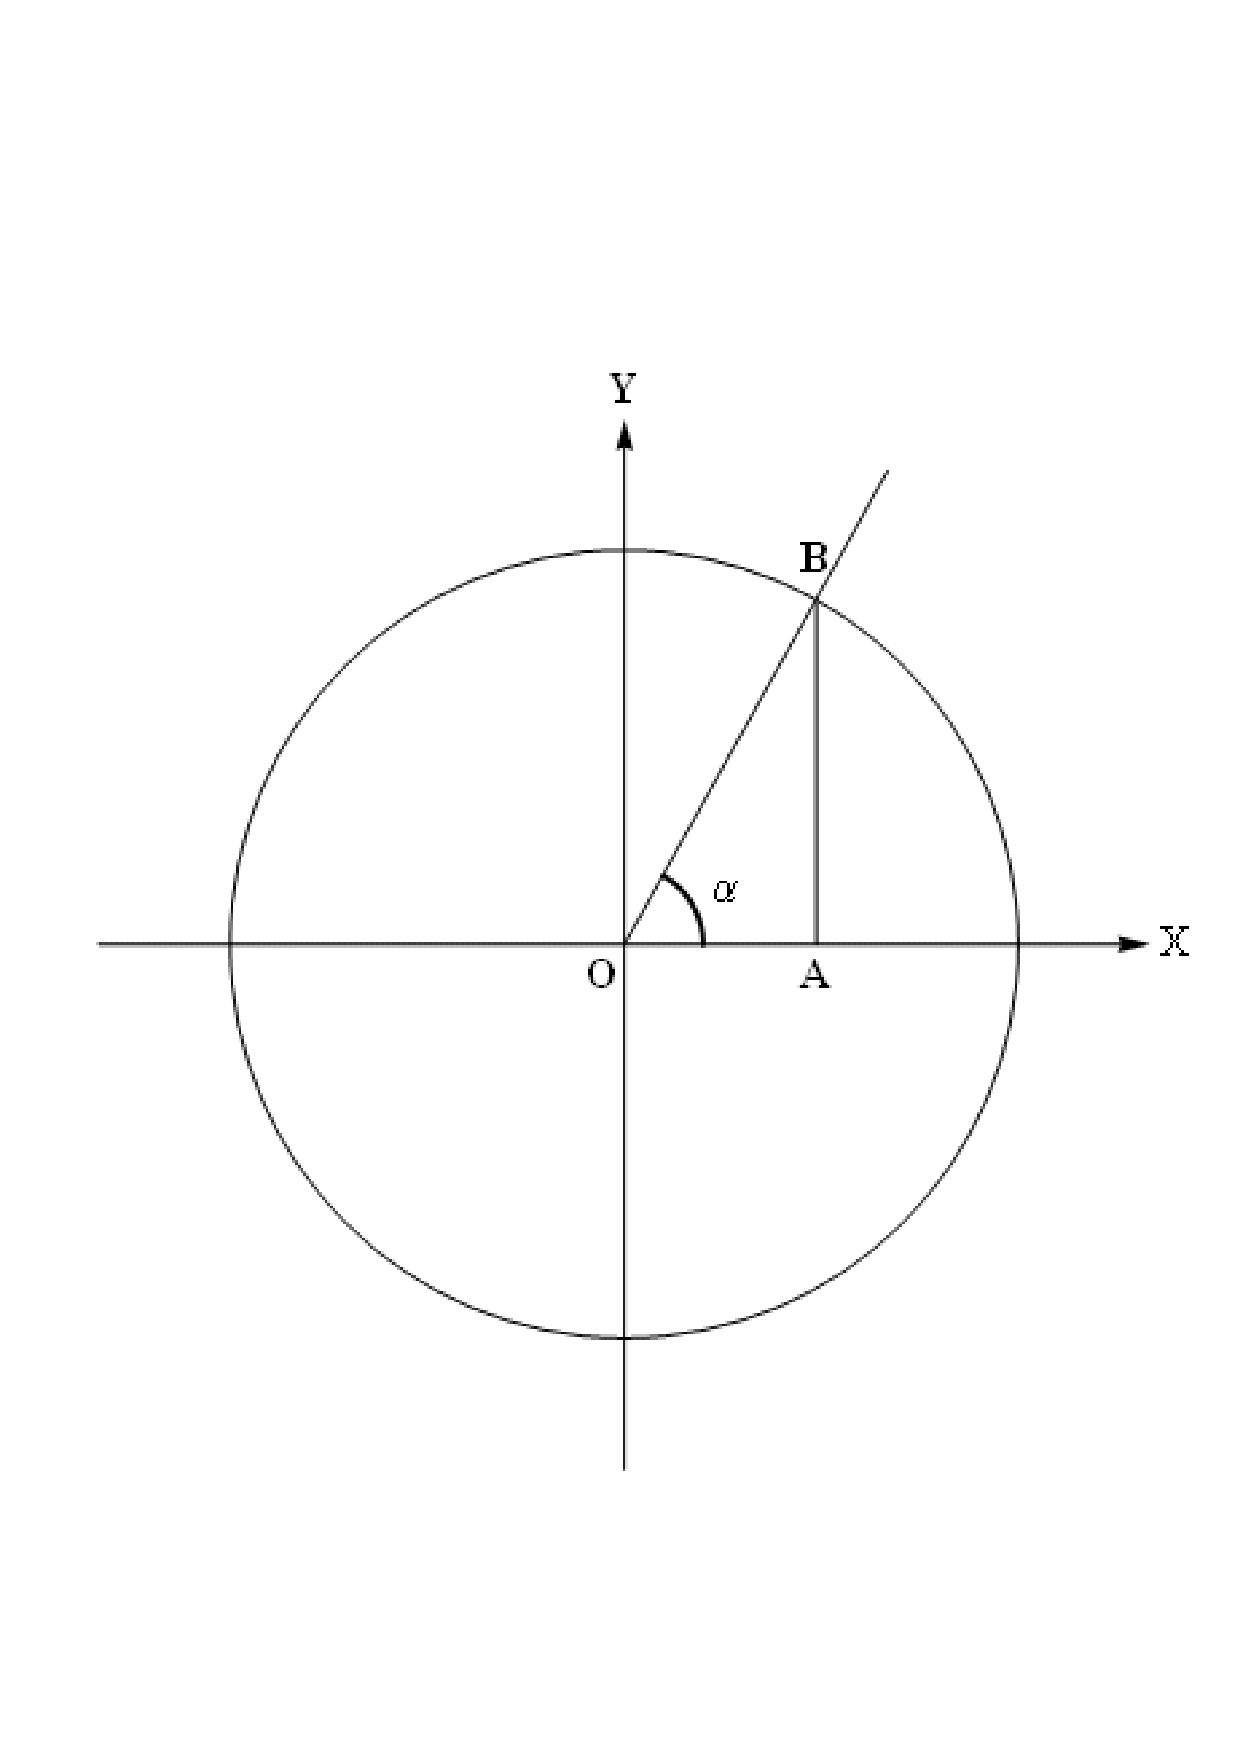
\includegraphics[width=0.48\textwidth]{trigonometry}
 \end{center}
 \caption{Единичная окружность}
 \label{pic:trig_circle}
\end{wrapfigure}
Введём систему декартовых
координат с нулём в центре окружности (точка $O$, рис.~\ref{pic:trig_circle}).
Отобразим числовую прямую на окружность,
а именно сопоставим ноль числовой прямой с точкой пересечения окружности и оси абсцисс (точка $A$).
Затем сопоставим точку $x$ числовой прямой с точкой на окружности, отложенной от
нулевой точки так, что длина полученной дуги окружности будет в точности равна $x$ (точка $B$).
Длина всей окружности равна $2\pi$ по определению числа $\pi,$ тогда очевидно,
что точки вида $x+2\pi k,~k\in \mathbb{Z}$ числовой прямой будут отображены в одну и ту же
точку на окружности. Значение угла $\angle BOA$ определим как длину дуги $\cup BOA.$ Теперь
определим тригонометрические функции.
\begin{definition}[Косинус]
$\cos x$ --- это $x$-координата точки $B.$
\end{definition}
\begin{definition}[Синус]
$\sin x$ --- это $y$-координата точки $B.$
\end{definition}
\begin{definition}[Тангенс]
$\tg x = \frac {\sin x}{\cos x}.$
\end{definition}
\begin{definition}[Котангенс]
$\ctg x = \frac {\cos x}{\sin x}.$
\end{definition}
Существуют такие функции, как $\sec x$ и $\csc x,$ но только бородатые старики,
запертые в подвалах университетов, помнят определение этих экзотических символов.
Самые базовые свойства тригонометрических функций мы рассмотрим в задачах, более
последовательно тригонометрия будет изложена в основном курсе математики ФМШ.
\subsection*{Задачи}
\begin{task}
Найдите период функций $\sin x,$ $\cos x,$ $\tg x,$ $\ctg x.$
\end{task}
\begin{solution}
$2\pi,~2\pi,~\pi,~\pi.$
\end{solution}
\begin{task}
Найдите область определения функций $\sin x,$ $\tg x.$
\end{task}
\begin{solution}
Проекция на ось $y$ определена всегда, поэтому
$\mathbb{D}\sin = \mathbb{R}.$
Функция $\cos x$ принимает значение $0$ при $x=\pi (k + 1/2), k \in \mathbb{Z}.$
Поэтому $\mathbb{D}\tg = \mathbb{R}\setminus\{\pi (k +1/2)\vert k\in\mathbb{Z}\}.$
\end{solution}
\begin{task}
Найдите область значений функций $\cos x,$ $\ctg x.$
\end{task}
\begin{solution}
Максимальное значение функции $\cos x$ --- $1$,
минимальное --- $-1,$ функция
\textit{непрерывна},
поэтому $\mathbb{E}\cos = [-1,~1].$
$\mathbb{E}\ctg = \mathbb{R}.$
\end{solution}
\begin{task}
Найдите значение функций $\sin x,$ $\tg x$
при $x =  0,$ 
$\pi/6,$ $\pi/4,$ $\pi/3,$ $\pi/2.$
\end{task}
\begin{solution}
$\sin x = 0,$ $1/2,$ $\sqrt 2/2,$ $\sqrt 3/2, 1.$
$\tg x = 0,$ $1/\sqrt 3,$ $1,$ $\sqrt 3,$ не определён.
\end{solution}
\begin{task}
Докажите следующие соотношения:
\begin{enumerate}
\item $\sin -x = -\sin x,$
\item $\sin (\pi/2-x) = \cos x,$
\item $\sin (x+\pi) = -\sin x,$
\item $\sin^2 x + \cos^2 x = 1.$
\end{enumerate}
\end{task}
\section{Понятие вектора}
Рассмотрим множество $\mathbb{V}$ элементов $\mathbf{v}.$ Пусть для всех $\mathbf{v}$ определена
бинарная операции (сложение) и операция умножения на скаляр (в нашем случае скаляром
будем считать элементом множества $\mathbb{R}$). Заданные операции удовлетворяют следующим
аксиомам 
($\mathbf{x},$ $\mathbf{y},$ $\mathbf{z} \in \mathbb{V},$ $\lambda, \mu \in \mathbb{R}$):
\begin{enumerate}
\item $\mathbf{x}+\mathbf{y} = \mathbf{y}+\mathbf{x},$
\item $\mathbf{x}+(\mathbf{y}+\mathbf{z}) = (\mathbf{x} + \mathbf{y}) + \mathbf{z},$
\item $\forall\mathbf{x}~\exists \mathbf{0} \in \mathbb{V}$ такой что $\mathbf{x}+\mathbf{0} = \mathbf{x},$
\item $\forall\mathbf{x}~\exists \mathbf{-x}\in\mathbb{V}$ такой что $\mathbf{x}+(\mathbf{-x})=\mathbf{0},$
\item $\lambda (\mu\mathbf{x}) = (\lambda \mu) \mathbf{x},$
\item $1\mathbf{x} = \mathbf{x},$
\item $(\lambda+\mu)\mathbf{x} = \lambda\mathbf{x} + \mu\mathbf{x},$
\item $\lambda (\mathbf{x} + \mathbf{y}) = \lambda \mathbf{x} + \lambda \mathbf{y}.$
\end{enumerate}
\begin{definition}[Векторное пространство]$\mathbb{V}.$\end{definition}
\begin{definition}[Вектор]$\mathbf{v} \in \mathbb{V}.$
 \label{def:vec}
\end{definition}
\begin{definition}[Линейная комбинация]
$\mathbf{L} = \sum\limits_{i=1}^{n}\lambda_i \mathbf{x}_i,$ $i \in \mathbb{N},$
$\lambda_i \in \mathbb{R},$ $\mathbf{x}_i\in\mathbb{V}.$
\end{definition}
\begin{definition}[Линейная независимость]
Система векторов $\{\mathbf{x}_i~\vert~\mathbf{x}_i\in \mathbb{V}\}$ является
линейнонезависимой, если $\mathbf{L}=0 \Leftrightarrow \forall i \therefore 1\le i\le n,$ $i\in\mathbb{N},$ 
$\lambda_i = 0.$
\end{definition}
\begin{definition}[Базис]
Система линейнонезависимых векторов $\{\mathbf{x}_i\}$ называется
базисом, если $\forall \mathbf{x} \in \mathbb{V}$ можно
представить в виде линейной комбинации $\{\mathbf{x}_i\}.$
\end{definition}
\begin{definition}[Размерность пространства]
$\dim \mathbb{V}$ --- число векторов в базисе.
\end{definition}
В физических задачах очень часто встречаются случаи, когда $\dim \mathbb{V} = 3.$
\begin{definition}[Скалярное произведение]
Бинарная операция $\langle \cdot \vert \cdot \rangle$ определена для всех
пар $\mathbf{x},$ $\mathbf{y} \in \mathbb{V},$ принимает значения из $\mathbb{R}$ и
удовлетворяет следующим условиям
при $\mathbf{x},$ $\mathbf{y},$ $\mathbf{z} \in \mathbb{V},$ $\lambda, \mu \in \mathbb{R}$:
\begin{enumerate}
\item $\langle \mathbf{x} \vert \lambda \mathbf{y} + \mu \mathbf{z} \rangle
 = \lambda \langle \mathbf{x} \vert \mathbf{y} \rangle
 + \mu \langle \mathbf{x} \vert \mathbf {z} \rangle,$
\item $\langle \mathbf{x} \vert \mathbf {y} \rangle
 = \langle \mathbf{y} \vert \mathbf {x} \rangle,$
\item $\langle \mathbf {x} \vert \mathbf {x} \rangle \ge 0,$
 причём $\langle \mathbf {x} \vert \mathbf {x} \rangle = 0
 \Leftrightarrow \mathbf {x} = \mathbf {0}.$
\end{enumerate}
\label{def:scalar_mul}
\end{definition}
\begin{definition}[Норма вектора]
$\lVert \mathbf{x}\rVert = \sqrt {\langle \mathbf {x} \vert \mathbf {x} \rangle}.$
\end{definition}
\begin{definition}[Ортонормированная система]
Система линейнонезависимых векторов $\mathbb{S}=\{\mathbf{x}_i~\vert~\mathbf{x}_i \in \mathbb{V}\}$
называется ортонормированной, если для любой пары $x_i,$ $x_j \in \mathbb{S}$
выполняется условие
$$\langle \mathbf {x_i} \vert \mathbf {x_j} \rangle = \left \{
\begin{matrix}
1,\text{если }i=j,\\
0,\text{если }i\ne j.\end{matrix}
\right.$$
\end{definition}
\begin{definition}[Проекция на вектор]
$$\mathbb{P}_\mathbf{v}\mathbf{x} = \frac {\langle\mathbf{x}\vert\mathbf{v}\rangle}
						{\langle\mathbf{v}\vert\mathbf{v}\rangle}\mathbf{v}$$
\end{definition}
\subsection*{Задачи}
\begin{task}
Направленный отрезок --- отрезок, крайние точки которого
указаны как <<начало>> и <<конец>>. Определим равенство двух
направленных отрезков как их параллельность, равенство их длин
и совпадение <<начала>> и <<конца>> при наложении друг на друга
параллельным образом.
$\amalg$ <<вектор>> $\vec{v}$ --- это класс равных между собой направленных отрезков.
Определим операцию сложения двух <<векторов>> как <<вектор>>,
полученный соединением <<начала>> второго <<вектора>> с <<концом>> <<первого>>,
<<начало>> результирующего вектора совпадёт тогда с <<началом>> первого <<вектора>>,
<<конец>> результирующего вектора совпадёт тогда с <<концом>> второго <<вектора>>.
Покажите, что такое определение корректно, то есть сумма двух <<векторов>>
не зависит от того, какие конкретно направленные отрезки будут соединяться.
\label{task:sum_vec}
\end{task}
\begin{solution}Очевидно.\end{solution}
\begin{task}
Определим умножение <<вектора>> $\vec{v}$ на скаляр $\lambda$
как вектор длины $\lvert \lambda \rvert \cdot \lVert \vec{v} \rVert$,
где $\lVert \cdot \rVert$ --- длина направленноего отрезка, представляющего
<<вектор>> $\vec{v}.$ $\lambda\vec{v}$ сонаправлен с $\vec{v},$ если
$\lambda \ge 0,$ противонаправлен иначе. Покажите корректность данного
определения.
\label{task:mul_vec}
\end{task}
\begin{solution}
Очевидно.
\end{solution}
\begin{task}Покажите, что определённое в задачах \ref{task:sum_vec}, \ref{task:mul_vec}
понятие <<вектора>> удовлетворяет определению \ref{def:vec}, то есть
<<вектор>> --- это вектор.
\end{task}
\begin{solution}
Очевидно.
\end{solution}
\begin{task}
Определим <<скалярное произведение>> <<векторов>> $\vec{x},$ $\vec{y}$
следующим образом:
$$\vec{x} \cdot \vec {y} = \lVert\vec{x} \rVert\cdot \lVert \vec{y} \rVert \cdot \cos \widehat{\vec{x}\vec{y}}$$
Покажите, что <<скалярное произведение>> --- это скалярное произведение (по определению \ref{def:scalar_mul}).
\end{task}
\begin{task}
$\amalg$ в двумерном линейном пространстве задан ортонормированный базис
$\{\mathbf{i},$ $\mathbf{j}\}.$ Разложите произвольный вектор $\mathbf{x}$
по этому базису (т.е. представьте $\mathbf{x}$ в виде линейной комбинации
векторов $\mathbf{i}$ и $\mathbf{j}.$ Рассмотрите также случай трёхмерного пространства,
$n-$мерного пространства.
\end{task}
\begin{solution}
Так как $\{\mathbf{i},$ $\mathbf{j}\}$ образуют базис, то
$\mathbf{x} = \lambda \mathbf{i} + \mu \mathbf{j}.$ В силу ортонормированности
базиса имеем
$\lambda = \frac{\langle\mathbf{x}\vert\mathbf{i}\rangle}
		{\langle\mathbf{i}\vert\mathbf{i}\rangle},$
$\mu = \frac{\langle\mathbf{x}\vert\mathbf{j}\rangle}
		{\langle\mathbf{j}\vert\mathbf{j}\rangle},$
$\mathbf{x} = \mathbb{P}_\mathbf{i}\mathbf{x}+
\mathbb{P}_\mathbf{j}\mathbf{x}.$

Остальные случаи получаются аналогичным образом:
$$\mathbf{x} = \sum\limits_{k=1}^{n}\mathbb{P}_{\mathbf{i}_k}\mathbf{x}
 = \sum\limits_{k=1}^{n}\frac{\langle\mathbf{x}\vert\mathbf{i}_k\rangle}
 		{\langle\mathbf{i}_k\vert\mathbf{i}_k\rangle}\mathbf{i}_k.$$
\end{solution}
\begin{task}
$\amalg$ в двумерном линейном пространстве задан ортонормированный базис
$\{\mathbf{i},$ $\mathbf{j}\}.$ Представьте произвольный вектор $\mathbf{x}$
из этого пространства через вектора $\mathbf{i},$ $\mathbf{j},$ норму
вектора $\lVert \mathbf{x}\rVert = \varrho$ и угол $\varphi$ между вектором $\mathbf{x}$ и
$\mathbf{i}.$
\end{task}
\begin{solution}
$\mathbf{x} = \varrho (\mathbf{i}\cos \varphi + \mathbf{j}\sin \varphi).$
\end{solution}
\begin{task}
Используя результат предыдущей задачи покажите, что
\begin{align*}
\sin(\alpha \pm \beta)& = \sin\alpha\cos\beta\pm\sin\beta\cos\alpha,\\
\cos(\alpha \pm \beta)& = \cos\alpha\cos\beta\mp\sin\beta\cos\alpha.
\end{align*}
\textbf{Подсказка.} Рассмотрите некий вектор $\mathbf{r}$, характеризованный
в базисе $\{\mathbf{i}, \mathbf{j}\}$ нормой $\varrho$ и углом $\alpha,$
в другом базисе $\{\mathbf{i}',\mathbf{j}'\},$ повёрнутом относительно начального
базиса на угол $\pm \beta.$
\end{task}
